\chapter{Modelo Matemático} \label{cap:modelo}

En este capítulo se presenta el marco teórico que sustenta este trabajo. Se introduce brevemente el concepto de turbulencia. Luego, se describen las ecuaciones, junto con las condiciones de borde, empleadas para modelar el sistema físico bajo análisis: fluido confinado entre placas paralelas sometido a un flujo de calor constante en las paredes. Asimismo, se definen las magnitudes estadísticas necesarias para el tratamiento de los datos obtenidos mediante simulaciones.

Por otra parte, se incluye un breve resumen del análisis de estabilidad lineal que constituye la base teórica para el cálculo numérico de los autovalores y autofunciones empleados en la construcción de las perturbaciones utilizadas para inestabilizar flujos con convección mixta. Estas perturbaciones se aplican en el Capítulo \ref{cap:transicion}, donde se analiza la transición temporal laminar–turbulenta.

\section{El concepto de turbulencia}

Como se menciona en el Capítulo \ref{cap:intro}, los flujos se clasifican, de manera general, en laminares, de transición y turbulentos. La mayoría de los flujos presentes en la naturaleza y en aplicaciones industriales son turbulentos, por lo que su estudio tiene un gran interés tanto en el ámbito científico como en el tecnológico. Algunos ejemplos de flujo turbulento se encuentran presentes en el movimiento de las nubes en el cielo, las corrientes oceánicas, el flujo sobre el ala de un avión o el flujo sobre el álabe de una turbina, entre muchos otros.

Todos estos flujos presentan un comportamiento aparentemente aleatorio y caótico, lo cual a menudo se refleja en las variaciones espaciales y temporales de las variables del flujo, tales como la velocidad y la temperatura. Las complejidades inherentes a la turbulencia dificultan su definición de forma concisa; por ello, en general, no es común dar una definición de turbulencia sino más bien presentar ciertos atributos canónicos \cite{smits2009lectures}:

\begin{itemize}
	
	\item \textbf{Tridimensionalidad.} La turbulencia es un fenómeno inherentemente tridimensional. 
	
	\item \textbf{Naturaleza no estacionaria.} Los flujos turbulentos evolucionan en el tiempo y se caracterizan por variaciones en magnitudes asociadas (velocidad, presión, temperatura, etc.).
	
	\item \textbf{Carácter multiescala.} La turbulencia involucra una amplia gama de escalas en el espacio y en el tiempo. 
	
	\item \textbf{Difusividad.} Se tiene una mezcla eficaz\footnote{El término ``mezcla eficaz'' se refiere a la capacidad de un flujo turbulento para mezclar y dispersar las diferentes propiedades del fluido de manera rápida y homogénea \cite{pope2001turbulent}.} de todas las propiedades del fluido (masa, velocidad, temperatura, concentración, etc.).

\end{itemize}

Por su relevancia práctica y su naturaleza aleatoria y compleja, este fenómeno ha sido objeto de un gran número de investigaciones teóricas y experimentales a lo largo de los últimos dos siglos. Incluso en la actualidad, se sigue estudiando con el objetivo de entender mejor su complejidad. En este contexto, el uso de la computación para resolver las ecuaciones que gobiernan la dinámica de fluidos ha adquirido un papel preponderante y se ha consolidado como una de las herramientas más utilizadas para el análisis de flujos turbulentos.

El rápido progreso de las computadoras de alto rendimiento permite que la \linebreak simulación numérica directa (\textit{Direct Numerical Simulation}, DNS) sea una herramienta fundamental para la investigación de la turbulencia \cite{moin1998direct}.{\linebreak}Esta permite calcular la solución tridimensional y no estacionaria de las ecuaciones de conservación involucradas. Al resolverse sin recurrir a modelos de turbulencia, estas simulaciones requieren una precisión numérica elevada para capturar todas las escalas del flujo \cite{pope2001turbulent}.

\section{Descripción del sistema bajo estudio} \label{sec:descripcion}

Se considera el sistema representado en la Figura \ref{fig:sistem_domain}, donde la dinámica de un fluido viscoso e incompresible sucede entre dos paredes paralelas infinitas ubicadas en $y=\pm d$. Esto constituye un canal vertical de placas paralelas donde ambas paredes están sometidas a un flujo de calor constante $q''_w$.

\begin{figure}[H]
 \centering
  \subfloat[]{
    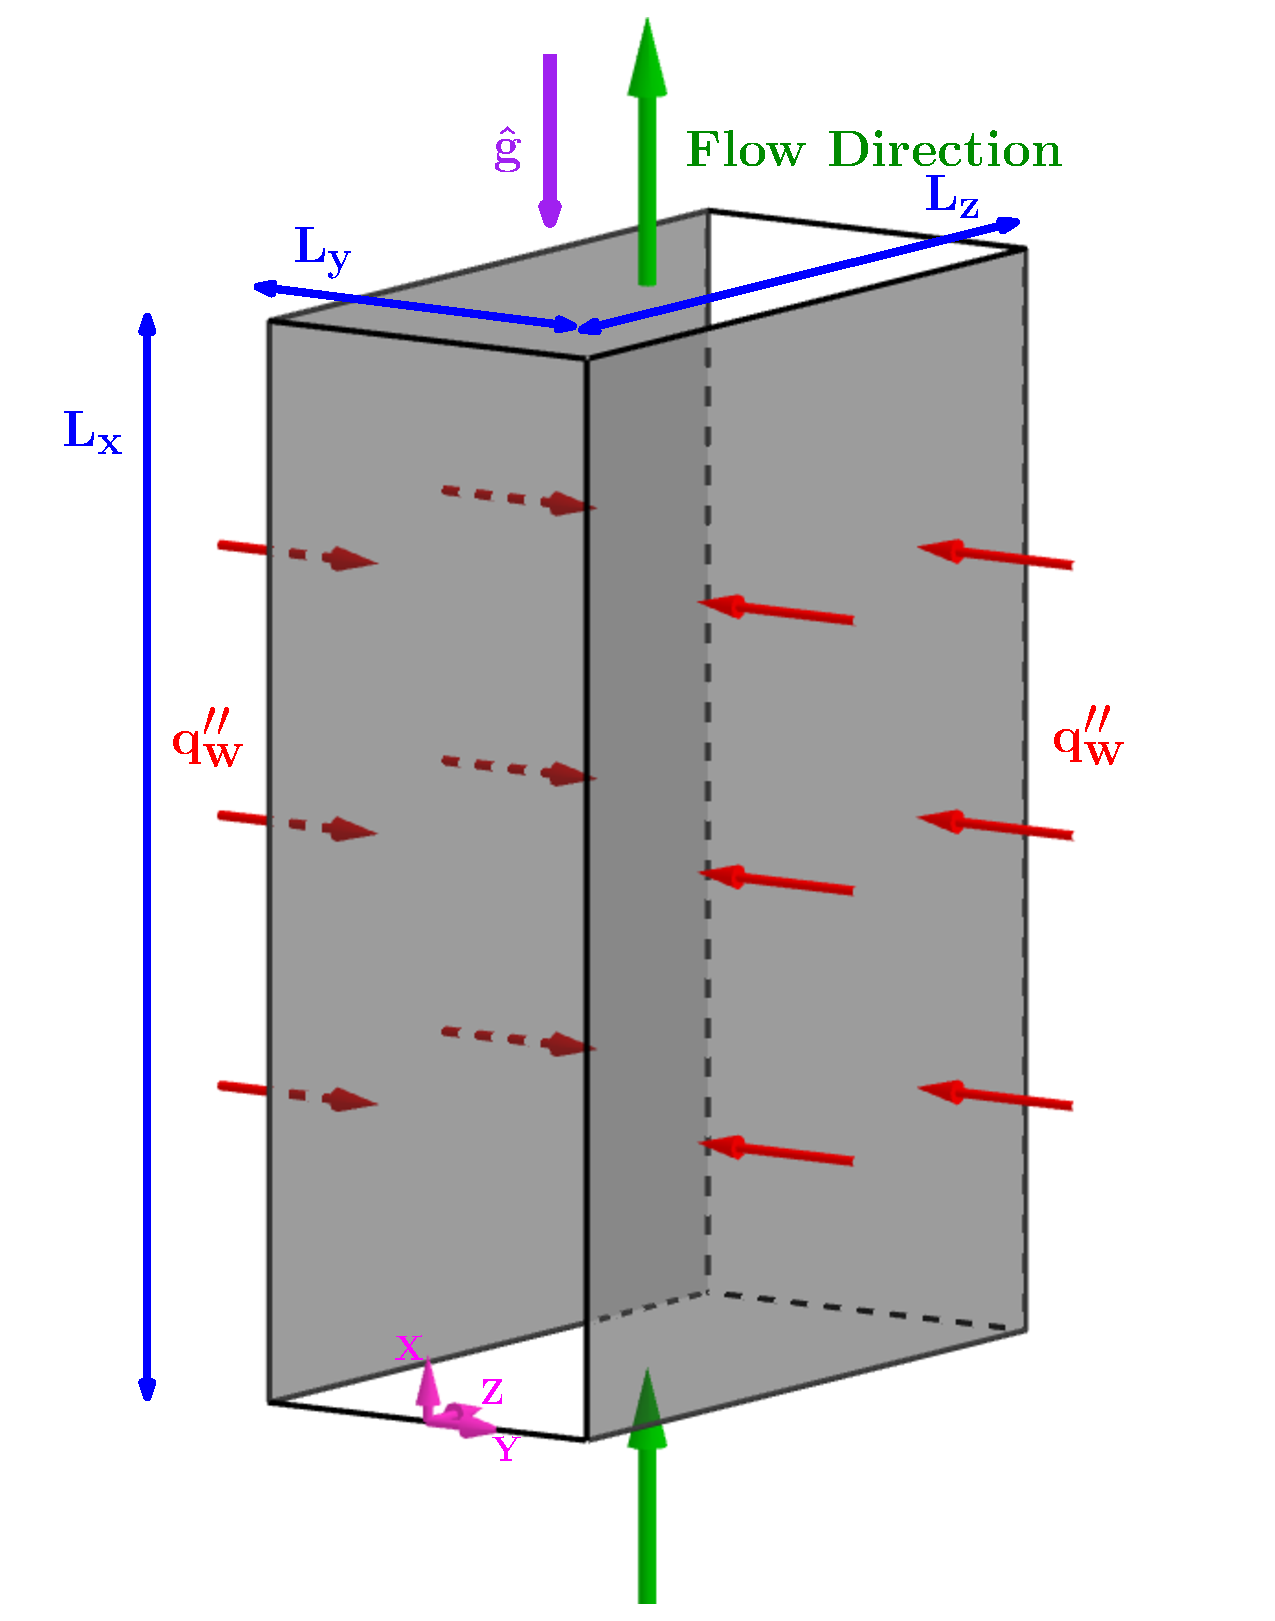
\includegraphics[width=0.49\textwidth]{figures/cap2/domain3d.eps}
    \label{fig:dom3d}}  
    \subfloat[]{
    \includegraphics[width=0.49\textwidth]{figures/cap2/domain2d.eps}
    \label{fig:dom2d}}  
 \caption{Esquema del sistema físico bajo análisis.} 
 \label{fig:sistem_domain}
\end{figure}

El flujo ocurre en la dirección paralela al eje $X$ (\textit{streamwise}) y su sentido es opuesto a la aceleración de la gravedad. Esta configuración se conoce como flujo ascendente o \textit{aiding flow}. Las ecuaciones de gobierno corresponden a los principios de conservación de masa, momento y energía \cite{zhou2024direct}. Las mismas se expresan en el recuadro \ref{eq:gob_system} donde $\rho$, $\mu$ y $\alpha_{T}$ son la densidad, la viscosidad dinámica y la difusividad térmica del fluido de trabajo, respectivamente. Por su parte, la variable $\mathbf{u}(x,y,z,t)$ corresponde al campo de velocidades, $T(x,y,z,t)$ es el campo de temperaturas y $\text{p}(x,y,z,t)$ el campo de presiones, donde $x,y,z$ son las coordernadas cartesianas y $t$ es el tiempo; por último, $\mathbf{g}$ es un vector que representa la aceleración de la gravedad.

\begin{equation}
        \boxed{ \begin{array}{lcc}
			  %\\
              &  \nabla \cdot \left( \rho \mathbf{u} \right) = 0 \\
              \vspace*{2mm}
              &  \frac{\partial \left( \rho \mathbf{u} \right)}{\partial t} + \mathbf{u} \cdot \nabla  \left( \rho \mathbf{u} \right) = -\nabla \text{p} + \mu \hspace{1mm} {\nabla}^2 \mathbf{u}  + \rho \hspace{1mm} \mathbf{g} \\
              \vspace*{2mm}
              &  \frac{\partial T}{\partial t} + \mathbf{u} \cdot \nabla T =  \alpha_{T} \hspace{1mm} \nabla^2 T  \\
              % \\
             \end{array}
               }
             \label{eq:gob_system}
\end{equation}

Este sistema físico admite soluciones completamente desarrolladas\footnote{Esto es: soluciones donde los perfiles de las cantidades involucradas expresadas en forma adimensional no dependen de la dirección \textit{streamwise}.}. No \linebreak obstante, la concepción del mismo supone dimensiones infinitas en las direcciones $X$ y $Z$. Debido a una limitación computacional evidente, nuestro modelo numérico no puede abarcar tales dimensiones. En ese sentido, el ``dominio infinito'' se reemplaza por un dominio acotado de dimensiones $L_x \times L_y \times L_z$ (Figura \ref{fig:dom3d}). Luego, se adoptan condiciones de borde periódicas (PBC) en la direcciones $X$ y $Z$ a fin de obtener dichas soluciones desarrolladas\footnote{Obsérvese, que al tratarse de flujos turbulentos (véase Sección \ref{sec:mag-stat}), el concepto de solución \linebreak desarrollada se aplica sobre perfiles promediados. En ese sentido, los perfiles completamente desarrollados son a su vez estadísticamente estacionarios.}. Estas condiciones de borde, definidas en las ecuaciones \ref{eq:pbc1} y \ref{eq:pbc2} (donde $\xi$ es un campo escalar arbitrario), pueden interpretarse como una prolongación del dominio finito que ``emula'' un dominio infinito mediante su repetición. Por su parte, la condición de flujo de calor constante en las paredes se impone como condiciones de Neumann (ecuación \ref{eq:neumann}).

\begin{align}
\xi(x=0,y,z,t) &= \xi(x=L_x,y,z,t)
\label{eq:pbc1} \\
\xi(x,y,z=0,t) &= \xi(x,y,z=L_z,t)
\label{eq:pbc2}
\end{align}

\begin{equation}
\kappa \hspace{0.5mm} \left. \frac{\partial T}{\partial y} \right\vert_{y=\mp d} = \pm q''_w \text{.}
\label{eq:neumann}
\end{equation}



Un análisis físico del problema bajo estudio muestra que no es posible imponer las condiciones \ref{eq:pbc1} y \ref{eq:pbc2} a las ecuaciones \ref{eq:gob_system}. Es decir, si se impone un flujo de calor constante en las paredes es esperable que la temperatura del fluido crezca en la dirección de la corriente. Análogamente, se entiende que no es posible imponer las condiciones de periodicidad al campo de presiones. Por lo cual, es necesario redefinir nuestras variables a fin de imponer condiciones de borde periódicas.

Primero se discute la variable de temperatura ($T$). Dado que se buscan soluciones desarrolladas se requiere que los perfiles de temperatura no modifiquen su forma con la coordenada \textit{streamwise}, y entonces estos se redimensionan con el incremento de energía recibido a través de las paredes. Esto equivale a suponer que la temperatura en la pared, promediada en el tiempo y en la dirección $Z$ (denotado por $\langle (\text{.})\rangle$), crece linealmente con la coordenada $x$, y por lo tanto: 

$$
\langle T_w \rangle = \mathcal{A} \hspace{0.5mm} x \text{ ,}
$$
siendo $\mathcal{A}$ una constante. Mediante un balance energético en el volumen de control $L_x \times L_y \times L_z$ (véase Apéndice \ref{apen:constante-A}), es posible demostrar que

$$\mathcal{A} = \frac{q''_w}{\rho_o  c_p U_b d} $$ 
donde $d$ es el semiancho del canal y $U_b$ la velocidad \textit{bulk} \cite{pope2001turbulent}.

Se realiza entonces el cambio de variable $T(x,y,z,t) = \langle T_w \rangle - \theta(x,y,z,t)$ para que $\theta(x,y,z,t)$ satisfaga las condiciones periódicas dadas por las relaciones \ref{eq:pbc1} y \ref{eq:pbc2}. Dicha modificación introduce un término fuente en la ecuación de conservación de energía:

\begin{equation}
\frac{ \partial \theta }{ \partial t } + \mathbf{u} \cdot \nabla \theta = \alpha_{T} \nabla^2 \theta + \mathcal{A} \hspace{0.5mm} u_x 
\label{eq:energy_pcb_source}
\end{equation}

Antes de discutir la periodicidad del campo de presiones es necesario introducir la aproximación que se utiliza para las variaciones de densidad en nuestro problema. Se emplea entonces la aproximación de Boussinesq que supone que los cambios de densidad en el fluido pueden despreciarse, excepto donde la densidad está multiplicada por la aceleración de la gravedad $\mathbf{g}$ \cite{kundu}. El término $\rho \hspace{1mm} \mathbf{g}$ de la ecuación de momento se reescribe considerando $\rho \equiv \rho(T)$ según la expresión \ref{eq:bussinesq}, donde $\rho_o \equiv \rho(T_R)$ es la densidad del fluido a una temperatura de referencia fija, $T_R$, y $ \langle \rho_w \rangle \equiv \rho(\langle T_w \rangle)$ es la densidad del fluido en la pared \cite{incropera}. Luego, la ecuación de momento queda reescrita como se expresa en la ecuación \ref{eq:mom_rewrite} siendo $\mathbf{\hat{e_g}}=(-1,0,0)$ y $C$ una constante que no depende de $x$.

\begin{equation}
\begin{aligned}
\rho(T) \mathbf{g} &= \rho_o \left[ 1 - \beta (T - T_R) \right] \mathbf{g} \\
				   &= \rho_o \left[ 1 - \beta ( \hspace{0.5mm} (\langle T_w \rangle - \theta) - T_R) \right] \mathbf{g} \\
 		           &= \rho_o \beta \theta \mathbf{g} + \rho_w \mathbf{g}
\end{aligned}
\label{eq:bussinesq}
\end{equation}

\begin{equation}
\frac{ \rho_o \hspace{0.5mm} \partial \mathbf{u}}{\partial t} + \mathbf{u} \cdot \nabla  \left( \rho_o \mathbf{u} \right) = -\nabla \left[ \text{p} + \left( \int \langle \rho_{w} \rangle \hspace{1mm} dx \right) \hspace{0.5mm} g + C \right] + \mu_o \hspace{1mm} {\nabla}^2 \mathbf{u}  + g \hspace{0.5mm} \rho_o \hspace{0.5mm} \beta \hspace{0.5mm} \theta \hspace{0.5mm} \mathbf{\widehat{e_g}},
\label{eq:mom_rewrite}  
\end{equation}

Ahora bien, se define $\text{p}^* = \left[ \text{p} + \left( \int \langle \rho_{w} \rangle \hspace{1mm} dx \right) \hspace{0.5mm} g + C \right] / \rho_o (U_o)^2 $, se examina con \linebreak atención la ecuación \ref{eq:mom_rewrite} y se asume que se buscan soluciones desarrolladas en el sentido estadístico $\langle \rangle$. Entonces, el término que contiene el gradiente de $\text{p}^*$ debe \linebreak depender de la coordenada \textit{streamwise}, mientras que los restantes dependen de la \linebreak coordenada normal a la pared (\textit{normalwise}). Por tanto, el gradiente de $\text{p}^*$ debe ser \linebreak constante\footnote{Observación: al buscar soluciones desarrolladas y tomando el promedio estadístico de la ecuación \ref{eq:mom_rewrite}, los campos de velocidad y de temperatura $\theta$ varían a lo largo de la dirección $Y$; por otro lado, el campo de presiones varía a lo largo de la dirección $X$. Entonces, es posible reacomodar la ecuación de momento de forma que $\text{LHS}(y)=\text{RHS}(x)=\text{cte}$ donde RHS (LHS) se refiere a \textit{Right Hand Side} (\textit{Left Hand Side}).}, o, de manera equivalente, $\langle \text{p}^* \rangle$ debe variar linealmente con la coordenada \linebreak $x$. Además, dado que el fluido de trabajo es impulsado por un caudal másico constante, para que $\text{p}^*$ sea periódica se debe imponer una fuerza volumétrica. Estas dos últimas cuestiones se representan por un solo término fuente en la ecuación de momento, $f \hspace{0.3mm} \mathbf{\widehat{e_x}}$, donde $f$ debe ser una constante en el espacio y variar con el tiempo de manera de mantener constante el caudal total.

Por otro lado, empleando la velocidad en el centro del canal $U_o$, el semiancho $d$ y la temperatura $T_o = \mathcal{A} \hspace{0.3mm} d $, el sistema de ecuaciones dimensional \ref{eq:gob_system} queda escrito en su forma adimensional como se muestra en el cuadro \ref{eq:gob_system_adim}. Los números adimensionales asociados a estas ecuaciones, se expresan en las relaciones \ref{eq:num_adim}. De izquierda a derecha, se tiene: el número de Reynolds, el número de Prandtl, el parámetro que acompaña al término boyante y al número de Richardson basado en el flujo de calor. Obsérvese que este último está expresado, a su vez, en términos de Richardson \textit{bulk} ($\text{Ri}_b$) que se define en base a la velocidad \textit{bulk} ($U_b$) y el ancho completo del canal ($2d$); este será utilizado a lo largo de los Capítulos \ref{cap:desarrollado} y \ref{cap:transicion}.


\begin{equation}
\boxed{
\begin{array}{l}
    \nabla^* \cdot \mathbf{u^*} = 0 \\
    \frac{\partial \mathbf{u^*}}{\partial t^*} + \mathbf{u^*} \cdot \nabla^* \mathbf{u^*} = 
    -\nabla \text{p}^* + \frac{1}{\text{Re}_o} \hspace{0.5mm} \nabla^{*2} \mathbf{u^*} + \Pi \hspace{0.5mm} \theta^* \hspace{0.5mm} \mathbf{\widehat{e_g}} + f \mathbf{\widehat{e_x}}  \\
    \frac{\partial \theta^*}{\partial t^*} + \mathbf{u^*} \cdot \nabla^* \theta^* = 
    \frac{1}{\text{Re}_o \hspace{0.5mm} \text{Pr}} \hspace{0.5mm} \nabla^{*2} \theta^* + u_x^* 
\end{array}
}
\label{eq:gob_system_adim}
\end{equation}

\begin{equation}
\text{Re}_o = \frac{\mu_o}{\rho_o \hspace{0.5mm} U_o \hspace{0.5mm} d } \quad ; \quad \text{Pr}= \frac{\mu_o}{\rho_o \hspace{0.5mm} \alpha_{T}} \quad ; \quad \Pi = \frac{\text{Ri}_o}{\text{Re}_o \hspace{0.5mm} \text{Pr}} \quad ; \quad \text{Ri}_o = \frac{g \hspace{0.5mm} \beta \hspace{0.5mm} q''_w \hspace{0.5mm} d^2}{k \hspace{0.5mm} U_o^2} = \frac{2}{9} \hspace{0.5mm} \text{Ri}_b
\label{eq:num_adim}
\end{equation}
%siendo Ra, el número de Rayleigh.

Nótese que en algunas de las referencias consideradas \cite{guo2022direct}, \cite{zhou2024direct}, \cite{tao1960}, al igual que en este trabajo, el sistema se modela \linebreak mediante las relaciones \ref{eq:gob_system_adim}; no obstante, ninguna de las referencias define de forma precisa la variable $\text{p}^*$.

Las condiciones de flujo de calor constante en las paredes se expresan, en su forma adimensional, en la ecuación \ref{eq:neumann_adim}. Sin embargo, estas condiciones pueden ser \linebreak aproximadas como condiciones de Dirichlet ya que al suponer que la temperatura de las paredes es constante\footnote{En este contexto, algunos autores \cite{kasagi1992direct} asumen que las fluctuaciones del flujo de calor y de la temperatura sobre la pared son pequeñas a fin de considerar que la temperatura en la misma es localmente isotérmica.} en el tiempo y en la dirección $Z$, y crece linealmente con la coordenada \textit{streamwise} de manera conocida se obtiene:
$$T(x,y=-d,z,t) = T(x,y=+d,z,t) \simeq \langle T_w \rangle \text{ .} $$

Este tipo de aproximación se conoce en la literatura como \textit{Mixed Boundary \linebreak Condition} (MBC) \cite{straub2019influence} y su forma adimensional se expresa en la ecuación \ref{eq:dirichlet_adim_theta}. En este trabajo se utiliza la aproximación MBC para imponer la condición de borde térmica dado que ha sido ampliamente evaluada y utilizada en el grupo de trabajo \cite{abregu2023dns}, \cite{szuban2023}, \cite{machaca2024}, y en diversas publicaciones científicas \cite{kawamura2000dns, kasagi1992direct}. Por último, para las componentes de la velocidad y del campo de presión, se adoptan condiciones de no deslizamiento y condiciones de Neumann homogéneas \cite{bartholomew2020xcompact3d}, respectivamente, en las paredes. 

\begin{align}
\begin{array}{l}
    \left. \frac{\partial \theta^*}{\partial y^*} \right\vert_{y^*=-1} = + \frac{2}{3} \text{Re}_o \hspace{0.5mm} \text{Pr} \\
    \left. \frac{\partial \theta^*}{\partial y^*} \right\vert_{y^*=+1} = - \frac{2}{3} \text{Re}_o \hspace{0.5mm} \text{Pr} 
\end{array}
\label{eq:neumann_adim}
\end{align}

\begin{equation}
\theta^*(x^*,y^*=0,z^*,t^*) = \theta^*(x^*,y^*=2,z^*,t^*) = 0
\label{eq:dirichlet_adim_theta}
\end{equation}



\subsection{Sumario de Ecuaciones}

\textbf{Ecuaciones de Gobierno:}
\begin{equation}
\begin{array}{l}
    \nabla^* \cdot \mathbf{u^*} = 0 \\
    \frac{\partial \mathbf{u^*}}{\partial t^*} + \mathbf{u^*} \cdot \nabla^* \mathbf{u^*} = 
    -\nabla \text{p}^* + \frac{1}{\text{Re}_o} \hspace{0.5mm} \nabla^{*2} \mathbf{u^*} + \frac{\text{Ri}_o}{\text{Re}_o \hspace{0.5mm} \text{Pr}} \hspace{0.5mm} \theta^* \hspace{0.5mm} \mathbf{\hat{g}} + f \mathbf{\widehat{e_x}}  \\
    \frac{\partial \theta^*}{\partial t^*} + \mathbf{u^*} \cdot \nabla^* \theta^* = 
    \frac{1}{\text{Pr}}\hspace{0.5mm}  \frac{1}{\text{Re}_o} \hspace{0.5mm} \nabla^{*2} \theta^* + u_x^* 
\end{array}
\label{eq:gob_system_res1}
\end{equation}

\textbf{Condiciones de borde.} Considérese $\xi= u^*_x, u^*_y, u^*_z, \text{p}^*, \theta^*$; entonces:
\begin{align}
&\xi(x^*=0,y^*,z^*,t^*) = \xi(x^*=L_x/d,y^*,z^*,t^*) 
	\label{eq:bc_1} \\
&\xi(x^*,y^*,z^*=0,t^*) = \xi(x^*,y^*,z^*=L_z/d,t^*) 
	\label{eq:bc_2} \\
&\theta^*(x^*,y^*=-1,z^*,t^*)       = \theta^*(x^*,y^*=+1,z^*,t^*) = 0
	\label{eq:bc_3} \\
&\mathbf{u^*}(x^*,y^*=-1,z^*,t^*)   = \mathbf{u^*}(x^*,y^*=+1,z^*,t^*) = 0
	\label{eq:bc_4} \\
&\partial_y \text{p}^*(x^*,y^*=-1,z^*,t^*) = \partial_y \text{p}^*(x^*,y^*=+1,z^*,t^*) = 0
	\label{eq:bc_5}
\end{align}


A lo largo de este trabajo, particularmente para el análisis de estabilidad lineal (Sección \ref{line_an}), se utiliza también la forma adimensional de las ecuaciones del trabajo de Chen \cite{chen1996linear} que se obtienen empleando el  semiancho del canal $d$, la velocidad \textit{bulk} $U_b$ y la temperatura $T_c = \text{Re} \hspace{0.5mm} \text{Pr} \hspace{0.5mm} \mathcal{A} \hspace{0.5mm} d$. Dichas ecuaciones se expresan en \ref{eq:gob_system_res2} donde se emplea el superíndice ``${\star}$'' para indicar esta variante adimensional. Las condiciones de borde son exactamente análogas a su forma adimensional de más arriba. Adicionalmente, aparece otro número adimensional conocido: el número de Rayleigh (Ra) basado en el flujo de calor y definido en la ecuación \ref{eq:Rayleigh}.

\begin{equation}
\begin{array}{l}
    \nabla^{\star} \cdot \mathbf{v^{\star}} = 0 \\
    \frac{\partial \mathbf{v^{\star}}}{\partial t^{\star}} + \mathbf{v^{\star}} \cdot \nabla^{\star} \mathbf{v^{\star}} = 
    -\nabla \text{p}^{\star} + \frac{1}{\text{Re}_b} \hspace{0.5mm} \nabla^{{\star}2} \mathbf{v^{\star}} + \frac{\text{Ra}}{\text{Re}_b} \hspace{0.5mm} \varphi^{\star} \hspace{0.5mm} \mathbf{\hat{g}} + f \mathbf{\hat{x}} \\
    \frac{\partial \varphi^{\star}}{\partial t^{\star}} + \mathbf{v^{\star}} \cdot \nabla^{\star} \varphi^{\star} = 
    \frac{1}{\text{Pr}}\hspace{0.5mm}  \frac{1}{\text{Re}_b} \hspace{0.5mm} \left[ \nabla^{{\star}2} \varphi^{\star} - v_x^{\star} \right]  
\end{array}
\label{eq:gob_system_res2}
\end{equation}

\begin{equation*}
\varphi^{\star} = -  \frac{\theta^*}{\text{Re}_o \hspace{0.5mm} \text{Pr}}  \quad ; \quad \mathbf{v^{\star}} = \frac{2}{3} \mathbf{u^*} \quad ; \quad \text{Re}_b = \frac{2}{3} \text{Re}_o
\end{equation*}  

\begin{equation}
\text{Ra} = \frac{g \hspace{0.5mm} \beta \hspace{0.5mm} q''_w \hspace{0.5mm} d^3}{c_p \hspace{0.5mm} \alpha_{T} \hspace{0.5mm} \mu_o \hspace{0.5mm} U_b} = \frac{\text{Ri}_b \hspace{0.5mm} \text{Re}_b}{2} 
\label{eq:Rayleigh}
\end{equation} 


\section{Magnitudes estadísticas de flujos turbulentos} \label{sec:mag-stat}

En flujos turbulentos, los campos como la velocidad son variables aleatorias \linebreak \cite{pope2001turbulent}. Supóngase que $\xi$ es un campo arbitrario asociado al sistema. Para una posición e instante determinados en un experimento (o simulación) repetible bajo las mismas condiciones, y sin dependencia entre repeticiones, el conjunto $\lbrace \xi^{(1)}, \xi^{(2)}, \cdots \rbrace$ puede considerarse de variables i.i.d. (independientes e idénticamente distribuidas). Entonces, el promedio en ensamble sobre $N$ repeticiones se define como 

\begin{equation*}
\langle \xi \rangle_N = \frac{1}{N} \sum^N_{n=1} \xi^{(n)} 
\end{equation*}
siendo $N$ muy grande. Si el sistema es estadísticamente estacionario, sus propiedades estadísticas no cambian con el tiempo; si es estadísticamente homogéneo, no varían con la posición; y si es ergódico \cite{moser2003}, el promedio en ensamble puede reemplazarse por el promedio en el tiempo y/o en el espacio (direcciones homogéneas). 

En problemas de turbulencia, los promedios y las fluctuaciones de las variables de interés son importantes, por lo que la descomposición de Reynolds \cite{pope2001turbulent, kundu} de la variable instantánea arbitraria $\xi$ puede representarse como un valor promedio $\langle \xi \rangle$ y una fluctuación $\xi^{\prime}$:

$$\xi = \langle \xi \rangle + \xi^{\prime}$$
donde $\langle (\text{.}) \rangle$ denota el promedio estadístico y $(\text{.})^{\prime}$ denota la parte fluctuante. 

Supongase entonces que $\eta$ es otra magnitud instantánea del flujo. El promedio de la multiplicación  de las fluctuaciones de $\xi$ y $\eta$ son cantidades de interés para la construcción de modelos de turbulencia \cite{pope2001turbulent}. Dichas cantidades nos indican qué tan correlacionadas están $\xi$ y $\eta$ entre sí. Estas se obtienen a partir del promedio de las magnitudes totales, ecuación \ref{eq:mag-cov}, donde se usa el hecho de que el promedio de una fluctuación es nulo y el promedio de otro promedio sigue siendo él mismo \cite{pope2001turbulent}. De esta manera, el promedio del producto de fluctuaciones $\langle \xi^{\prime} \eta^{\prime} \rangle$ queda expresado en la ecuación \ref{eq:fluct-corr}.

\begin{equation}
\begin{aligned}
\langle \xi \eta \rangle &= \langle (\langle \xi \rangle + \xi^{\prime}) (\langle \eta \rangle + \eta^{\prime}) \rangle \\
                         &= \langle \xi \rangle \langle \eta \rangle + \langle \xi^{\prime} \eta^{\prime} \rangle
\end{aligned}
\label{eq:mag-cov}
\end{equation}

\begin{equation}
\langle \xi^{\prime} \eta^{\prime} \rangle = \langle \xi \eta \rangle - \langle \xi \rangle \langle \eta \rangle
\label{eq:fluct-corr}
\end{equation}

Algunas cantidades importantes que aparecen en las ecuaciones promediadas de conservación (ecuaciones RANS \cite{kundu}) son:

\begin{itemize}
	\item $\langle u^{\prime}_i u^{\prime}_j \rangle$: componentes del tensor de Reynolds con $i,j=x,y,z$;
	\item $\langle \theta^{\prime} u^{\prime}_i \rangle$: flujos turbulentos de calor en la dirección $i$, con $i=x,y,z$;
	\item $\langle \theta^{\prime} \theta^{\prime} \rangle$: varianza de la temperatura;

	\item otra magnitud utilizada ampliamente a lo largo de este trabajo es la energía cinética turbulenta $\kappa$ (o TKE) definida como la mitad de la traza del tensor de Reynolds, esto es, 

\begin{equation}
\kappa = \frac{1}{2} \left[ \langle u^{\prime}_x u^{\prime}_x \rangle + \langle u^{\prime}_y u^{\prime}_y \rangle + \langle u^{\prime}_z u^{\prime}_z \rangle \right] \text{.}
\label{eq:tke}
\end{equation}

\end{itemize}


\section{Teoría de Estabilidad Lineal} \label{line_an}

La evolución de un flujo laminar a uno turbulento (transición laminar-turbulenta) es crucial en ingeniería ya que las características del mismo varían notablemente entre estos regímenes. Por ejemplo, como se mencionó, los coeficientes de fricción y de convección aumentan considerablemente al pasar de un régimen laminar a uno turbulento \cite{machaca2024}. Las ecuaciones de Navier–Stokes admiten ambas soluciones, lo que implica que el tipo de flujo y su evolución dependen de las perturbaciones y las condiciones impuestas sobre el sistema. 

Para analizar la estabilidad lineal y predecir cómo cambiará el flujo al ser perturbado, es indispensable conocer el flujo base. Sobre ese estado se introducen las perturbaciones que desencadenan inestabilidades y conducen a la transición. En este trabajo se adopta como flujo base al flujo laminar completamente desarrollado. 


\subsection{Flujo Base} \label{sec:fbase}

Si el flujo está completamente desarrollado, tanto térmica como hidrodinámicamente, y es laminar, entonces es posible redefinir los campos de interés para que dependan solamente de la variable $y^{\star}$. El sistema de ecuaciones \ref{eq:gob_system_res2} puede reducirse a la ecuación de momento en la dirección $X$ y a la ecuación de energía \cite{chen1996linear}, las cuales quedan expresadas de la forma 

\begin{align}
&\frac{d \text{p}^{\star} }{d x^{\star}} = \frac{\text{Ra}}{\text{Re}_b } \Phi^{\star} + \frac{1}{\text{Re}} \frac{d^2 V^{\star}_x}{d {y^{\star}}^2}, \\
&\frac{d^2 \Phi^{\star}}{ d {y^{\star}}^2 } =  V^{\star}_x \text{.}
\label{eq:base1}
\end{align}
El perfil de velocidad y de temperatura admiten las condiciones de borde \linebreak  $V^{\star}_x({y^{\star}}= \pm 1) = \Phi^{\star} ({y^{\star}}= \pm 1) = 0 $. Las soluciones para un flujo asistido por fuerzas \linebreak  boyantes ($\text{Ra}>0$) están dadas por las expresiones \ref{eq:vel_asist_boyant} y \ref{eq:theta_asist_boyant}, mientras que para un flujo donde las fuerzas boyantes son opuestas ($\text{Ra}<0$), las soluciones quedan definidas por las ecuaciones \ref{eq:vel_opo_boyant} y \ref{eq:theta_opo_boyant} \cite{chen1996linear}. Obsérvese que el único parámetro relevante aquí es el número de Rayleigh.
\small{
\begin{equation}
V^{\star}_x = \frac{-E}{\sqrt{\text{Ra}}} \frac{\sinh(\kappa(1+y^{\star}))\sin(\kappa(1-y^{\star})) + \sinh(\kappa(1-y^{\star}))\sin(\kappa(1+y^{\star})) }{\cosh(2\kappa) + \cos(2\kappa)}
\label{eq:vel_asist_boyant}
\end{equation}

\begin{equation}
\Phi^{\star} = \frac{E}{\text{Ra}} \left[ 1 - \frac{\cosh(\kappa(1+y^{\star}))\cos(\kappa(1-y^{\star})) + \cosh(\kappa(1-y^{\star}))\cos(\kappa(1+y^{\star}))}{\cosh(2\kappa) + \cos(2\kappa)} \right] 
\label{eq:theta_asist_boyant}
\end{equation}

\begin{equation}
V^{\star}_x = \frac{F}{2 m^2} \left( \frac{\cosh(m y^{\star})}{\cosh(m)} - \frac{\cos(m y^{\star})}{\cos(m)} \right) 
\label{eq:vel_opo_boyant}
\end{equation}

\begin{equation}
\Phi^{\star} = \frac{F}{2 m^4} \left( \frac{\cosh(m y^{\star})}{\cos(m)} + \frac{\cos(m y^{\star})}{\cos(m)} - 2 \right) 
\label{eq:theta_opo_boyant}
\end{equation}

\begin{equation*}
\kappa = \frac{\text{Ra}^{-1/4}}{\sqrt{2}} \quad ; \quad m = (-\text{Ra})^{1/4} \quad ; \quad F = \frac{2 m^3}{\tanh(m)-\tan(m)} \quad ; \quad
\end{equation*}

\begin{equation*}
E= -2 \kappa \hspace{1mm} \text{Ra}^{1/2} \hspace{1mm} \frac{\cosh(2\kappa) + \cos(2\kappa)}{\sinh(2\kappa) - \sin(2\kappa)} 
\end{equation*}
}
Cabe mencionar que estas soluciones se utilizan para validar la herramienta numérica \linebreak Xcompact3D. Si el lector lo desea, puede apreciar las gráficas de dichas soluciones en la Sección \ref{sec:mix-laminar}.  


\subsection{Análisis de Estabilidad Lineal} \label{sec:estabilidad}

Dos motivaciones principales para estudiar la estabilidad de los fluidos son: comprender el proceso de transición de un flujo laminar a uno turbulento, y predecir el inicio de dicha transición. El análisis de estabilidad lineal permite evaluar cómo se comporta un flujo ante perturbaciones, identificando los mecanismos que pueden inducir transiciones. En ese sentido, condiciones como un número de Reynolds inferior a un valor crítico garantizan la estabilidad de un flujo laminar suave \cite{drazin2004hydrodynamic}. Sin embargo, en ocasiones, las perturbaciones crecen hasta alcanzar amplitudes finitas y establecer nuevos equilibrios estacionarios, que pueden volverse inestables a su vez y evolucionar hacia un régimen turbulento. 

El enfoque parte de las ecuaciones de gobierno \ref{eq:gob_system_res2} donde se han omitido los superíndices ``${\star}$'' para simplificar la notación. La idea consiste en suponer que los campos solución \linebreak ($\mathbf{v}$, $\text{p}$, $\varphi$) pueden descomponerse como un flujo base más una perturbación:

\begin{align}
\mathbf{v} &= \mathbf{V} + \widetilde{\mathbf{v}} \\
\text{p} &= P + \widetilde{p} \\
\varphi &= \Phi + \widetilde{\varphi}
\end{align}  
donde las letras mayúsculas hacen referencia al flujo base laminar y aquellas letras con $\widetilde{(\text{.})}$ a las perturbaciones. 

Despreciando términos de segundo orden, esto es, productos de perturbaciones, y \linebreak asumiendo que los flujos base son los flujos laminares desarrollados $\mathbf{V} = (V_x(y),0,0)$ y $\Phi \equiv \Phi(y)$, es posible expresar las ecuaciones que describen la dinámica de $\widetilde{\mathbf{v}}$, $\widetilde{p}$ y $\widetilde{\varphi}$ de la siguiente forma: 

\begin{align}
&\nabla \cdot \mathbf{\widetilde{v}} = 0
\label{eq:pertub_continuity} \\
&\partial_t \mathbf{\widetilde{v}} + V_x \hspace{1mm} \partial_x \mathbf{\widetilde{v}} + {\widetilde{v_y}} \partial_y V_x \hspace{1mm} \mathbf{\hat{e_x}} = - \nabla \widetilde{p} + \frac{1}{\text{Re}_b} \hspace{1mm} \nabla^2 \mathbf{\widetilde{v}} + \frac{\text{Ra}}{\text{Re}_b} \hspace{1mm} \widetilde{\varphi} \hspace{1mm}  \mathbf{\widehat{e_x}} 
\label{eq:pertub_momentum} \\
&\partial_t {\widetilde{\varphi}} + V_x \hspace{1mm} \partial_x {\widetilde{\varphi}} + {\widetilde{v_y}} \partial_y \Phi \hspace{1mm} = \frac{1}{\text{Re}_b \hspace{1mm} \text{Pr}} \left[ \nabla^2 \widetilde{\varphi} - \widetilde{v_x} \right]
\label{eq:pertub_energy} 
\end{align} 

Luego, aplicando el operador divergencia a la ecuación \ref{eq:pertub_momentum} es posible encontrar una expresión para el Laplaciano de la presión:

\begin{equation}
- \nabla^2 \widetilde{p} = 2 \hspace{1mm} \partial_x \widetilde{v_y} \hspace{1mm} \partial_y V_x - \frac{\text{Ra}}{\text{Re}_b} \partial_x \widetilde{\varphi} \text{.}
\label{eq:pressure_eigen}
\end{equation}
A continuación, aplicando el operador Laplaciano a la componente $y$ de la ecuación \ref{eq:pertub_momentum} es posible eliminar el término que involucra la presión, resultando en la siguiente expresión:

\begin{equation}
\left\lbrace \left[ \partial_t + V_x \partial_x \right] \nabla^2 - D^2(V_x) \partial_x - \frac{1}{\text{Re}_b} \nabla^4 \right\rbrace \widetilde{v_y} = - \frac{\text{Ra}}{\text{Re}_b} \hspace{1mm} \partial_{xy} \widetilde{\varphi} \text{ ,}
\label{eq:eigensis_ec1}
\end{equation}
donde $D^j \equiv \partial^j_y$. 

Para la descripción completa de las perturbaciones se utiliza la componente $y$ de la vorticidad, $\widetilde{\eta} \equiv \partial_z \widetilde{v_x} - \partial_x \widetilde{v_z}$, cuya dinámica está dada por la ecuación \ref{eq:eigensis_ec2}.

\begin{equation}
 \left[ \partial_t + V_x \partial_x - \frac{1}{\text{Re}_b} \nabla^2  \right] \widetilde{\eta}  +  D(V_x) \hspace{1mm} \partial_z \widetilde{v_y} = \frac{\text{Ra}}{\text{Re}_b} \hspace{1mm} \partial_{z} \widetilde{\varphi}
\label{eq:eigensis_ec2}
\end{equation}

Así, las ecuaciones \ref{eq:pertub_energy}, \ref{eq:eigensis_ec1} y \ref{eq:eigensis_ec2} constituyen un sistema de EDP\footnote{Ecuaciones en Derivadas Parciales.} de tres ecuaciones con tres campos incógnitas. A partir de los campos escalares $\widetilde{\eta}$ y $\widetilde{v_y}$, utilizando la ecuación \ref{eq:pertub_continuity} y la definición de $\widetilde{\eta}$ es posible hallar los campos $\widetilde{v_x}$ y $\widetilde{v_z}$. Asimismo, empleando la ecuación \ref{eq:pressure_eigen} y los campos $\widetilde{v_y}$ y  $\widetilde{\varphi}$ es posible hallar el campo de presión  $\widetilde{p}$. 

Las soluciones a dicho problema se proponen como ondas planas tridimensionales. Si $\widetilde{\xi}$ es una perturbación cualquiera, entonces, se escribe de la siguiente forma arbitraria

\begin{equation}
\widetilde{\xi} = \hat{\xi}(y) \hspace{1mm} e^{i \left[ \alpha x + \beta z - \alpha c t \right]} \text{ ,}
\label{eq:waves3d}
\end{equation}
donde $c$  es la velocidad de fase, y $\alpha$ y $\beta$ son los números de onda en la dirección $X$ y $Z$, respectivamente; por otro lado se define $\omega \equiv \alpha c$ como la frecuencia angular. 

Si el crecimiento de la perturbación ocurre en el tiempo, se denomina transición temporal \cite{machaca2024}. Aquí, $c$ es la velocidad de fase compleja ($c \equiv c_r + i \hspace{0.5mm} c_i$) y la frecuencia $\omega$ es también una cantidad compleja ($\omega \equiv \omega_r + i \hspace{0.5mm} \omega_i$). En ese sentido: $\alpha$, $\beta$, $c_r$, $c_i$, $\omega_r$ y $\omega_i$ son números reales. Además, la perturbación crece o decae en el tiempo de acuerdo al término $e^{\alpha c_i t}$ dependiendo del signo de $c_i$: 

\begin{itemize}
\item[$\blacklozenge$] Si $\alpha c_i > 0$ entonces las perturbaciones crecen en el tiempo. El flujo se vuelve inestable.

\item[$\blacklozenge$] Si $\alpha c_i < 0$ entonces las perturbaciones decaen exponencialmente en el tiempo y la perturbación se atenúa. El flujo se vuelve estable.
\end{itemize}

Por otro lado, si el crecimiento de las perturbaciones ocurre en el espacio, por ejemplo a lo largo de la dirección $X$, entonces se denomina transición espacial \cite{machaca2024}. Aquí $c$, $\omega$ y $\beta$ son números reales, mientras que $\alpha$ es un número complejo ($\alpha = \alpha_r + i \alpha_i$). En este sentido:

\begin{itemize}
\item[$\blacklozenge$] Si $\alpha_i < 0$ entonces las perturbaciones crecen en el espacio, en la dirección de la \linebreak corriente. El flujo se vuelve inestable.

\item[$\blacklozenge$] Si $\alpha_i > 0$ entonces las perturbaciones decaen exponencialmente en el espacio y la pertubación se atenúa. El flujo se vuelve estable.
\end{itemize}

%donde $c \equiv c_r + i \hspace{0.5mm} c_i$ es la velocidad de fase compleja, $\alpha$ y $\beta$ son el número de onda en la dirección de la corriente $X$ y en la dirección $Z$, respectivamente; por otro lado, $\omega \equiv \alpha c$ es la frecuencia angular compleja. Además, $\alpha$, $\beta$, $c_r$ y $c_i$ son números reales. 

En este trabajo se considera únicamente la transición temporal. En este contexto, al reemplazar las soluciones tipo \ref{eq:waves3d} en el sistema de ecuaciones, se obtiene un problema de autovalores generalizado de la siguiente forma:

%En este sentido, dado que se busca y se estudia la transición temporal, se distinguen dos casos \cite{szuban2023}:
%
%\begin{itemize}
%\item[$\blacklozenge$] Si $\alpha c_i > 0$ entonces las perturbaciones crecen en el tiempo. El flujo se vuelve inestable.
%
%\item[$\blacklozenge$] Si $\alpha c_i < 0$ entonces las perturbaciones decaen exponencialmente en el tiempo y la pertubación se atenúa. El flujo se vuelve estable.
%\end{itemize}



\begin{equation}
\begin{bmatrix}
a_{11} & a_{12} & 0 \\[4pt]
a_{21} & a_{22} & a_{23} \\[4pt]
a_{31} & a_{32} & a_{33}
\end{bmatrix}
\,\begin{bmatrix}
\widehat{v_y} \\[4pt]
\widehat{\varphi} \\[4pt]
\widehat{\eta}
\end{bmatrix}
\;=\; i \omega
\,\begin{bmatrix}
  b_1 & 0 & 0 \\[4pt]
    0 & 1 & 0 \\[4pt]
    0 & 0 & 1
\end{bmatrix}
\,\begin{bmatrix}
\widehat{v_y} \\[4pt]
\widehat{\varphi} \\[4pt]
\widehat{\eta}
\end{bmatrix} \text{ ,}
\label{eq:eigensistem-general}
\end{equation}

\begin{align*}
a_{11} &= \frac{1}{\text{Re}_b} \left[ D^2 - k^2 \right]^2 - i \alpha \left( V_x \left[ D^2 - k^2 \right] + D^2(V_x)\right) \hspace{2mm} ; \hspace{2mm} a_{12} = -\left[ i \alpha \frac{\text{Ra}}{\text{Re}_b} D \right] \\
a_{21} &= \frac{i \alpha}{\text{Re}_b \hspace{1mm} \text{Pr} \hspace{1mm} k^2} D + D(\Phi) \hspace{2mm} ; \hspace{2mm} a_{22} = \frac{-1}{\text{Re}_b \hspace{1mm} \text{Pr} } \left[ D^2 - k^2 \right] + i \alpha V_x  \hspace{2mm} ; \hspace{2mm} a_{23} = \frac{\beta}{\text{Re}_b \hspace{1mm} \text{Pr} \hspace{1mm} k^2} \\
a_{31} &= \beta D(V_x) \hspace{2mm} ; \hspace{2mm} a_{32} = - \beta \frac{\text{Ra}}{\text{Re}_b}  \hspace{2mm} ; \hspace{2mm} a_{33} = -\frac{1}{\text{Re}_b} \left[ D^2 - k^2 \right] + i \alpha V_x \\
b_1    &= - \left[ D^2 - k^2 \right] \hspace{2mm} ; \hspace{2mm} k^2 = \alpha^2 + \beta^2 \\
\end{align*}
donde $\widehat{\eta} := \beta \hspace{0.5mm} \widehat{v_x} - \alpha \hspace{0.5mm} \widehat{v_z}$. A partir de las condiciones de borde \ref{eq:bc_1} - \ref{eq:bc_5}, las autofunciones $\widehat{v_y}(y)$, $\widehat{\varphi}(y)$, $\widehat{\eta}(y)$ deben satisfacer las condiciones:

\begin{equation}
\widehat{v_y}(y) = D(\widehat{v_y}) = \widehat{\varphi}(y) = \widehat{\eta}(y) = 0 \quad \text{en} \quad y= \pm 1
\label{eq:eigensis-ci}
\end{equation} 

La resolución de este problema de autovalores generalizado se realiza empleando una estrategia numérica la cual se detalla en el Capítulo \ref{cap:numerico}. 

\subsection{Mecanismos de Inestabilidad} \label{sec:mecanismo}

A continuación, la construcción de las condiciones iniciales que se consideran en \linebreak esta subsección se basan en el concepto de inestabilidad secundaria que ha sido utilizado por el grupo de trabajo en el caso de convección forzada. Allí, se perturba el flujo \linebreak laminar con una onda bidimensional más un par de ondas oblicuas \cite{machaca2024}, \cite{schmid}. Cabe destacar que esta estrategia también ha sido empleada en otros trabajos donde se estudian flujos en convección mixta \cite{chen2003direct}.  

En el caso de un flujo Poiseuille entre placas paralelas con convección forzada, se tiene, según la teoría de estabilidad lineal, que el flujo es estable para números de Reynolds menores que $\text{Re}_{\text{crit}}=5772$ \cite{orszag1971accurate}. Sin embargo, los experimentos reales muestran que el flujo puede inestabilizarse para $\text{Re} < \text{Re}_{\text{crit}}$, como es el caso del experimento realizado por \cite{kao1970experimental}, quienes encontraron un número de Reynolds crítico $\text{Re}_{\text{crit}}= 975$. 

En vista de que en los experimentos reales el flujo se inestabiliza a $\text{Re} < 5772$, muchos investigadores abarcaron el problema  de forma numérica. Por ejemplo, Orszag y Kells \cite{orszag1980transition} lograron inestabilizar el flujo para  $\text{Re} \approx 1000$ mediante la introducción de perturbaciones tridimensionales de pequeña amplitud. Estas perturbaciones tridimensionales dan lugar a lo que se conoce como inestabilidad secundaria.

La teoría de inestabilidad secundaria se ocupa del análisis de estabilidad de estados estacionarios o cuasi-estacionarios que resultan de la inestabilidad primaria. Esta última aborda la primera etapa del proceso de transición: el crecimiento de las ondas bidimensionales (2D) de Tollmien–Schlichting (TS) \cite{tollmien1935, schlichting1933} que se propagan en la dirección de la corriente. Cuando la amplitud de la onda TS excede cierto umbral, las perturbaciones tridimensionales (3D) comienzan a amplificarse \cite{schmid}. 

\textbf{En concreto:} para $\text{Re} < \text{Re}_{\text{crit}}$, la condición inicial que se impone al flujo tiene la forma de la ecuación \ref{eq:init_con_1} donde $\mathbf{V}=(V_x(y),0,0)$.

\begin{equation}
\begin{aligned}
\mathbf{v}(x,y,z,t=0) &= \mathbf{V} + \widetilde{\mathbf{v}} \\
\phi(x,y,z,t=0) &= \Phi +  \widetilde{\varphi} 
\end{aligned}
\label{eq:init_con_1}
\end{equation}
La condición inicial considerada para el crecimiento de la perturbación en el tiempo, se \linebreak construye como la suma del flujo base y la perturbación bidimensional compuesta por una onda 2D del tipo $\widehat{\xi}(y) \hspace{0.5mm} e^{i \hspace{0.5mm} \alpha_{2D} \hspace{0.5mm} x }$ (inestabilidad primaria). Luego se produce una saturación no lineal de la onda 2D mediante la adición de un par de ondas tridimensionales oblicuas del tipo $\widehat{\xi}(y) \hspace{0.5mm} e^{i \hspace{0.5mm} \alpha_{3D} \hspace{0.5mm} x \pm \beta z  }$ (inestabilidad secundaria). Así, la forma funcional de las perturbaciones $\widetilde{\mathbf{v}}$ y $\widetilde{\mathbf{\varphi}}$ se expresa en las ecuaciones \ref{eq:init_con_2} y \ref{eq:init_con_3}, respectivamente. Allí, $A_{2D}$ corresponde a la \linebreak amplitud de la perturbación bidimensional y $A_{3D}$ corresponde a la amplitud total del par de ondas tridimensionales. Las autofunciones $\widehat{\mathbf{v^{}_{2D}}}(y)$, $\widehat{\mathbf{v^{}_{3D}}}(y)$, $\widehat{\varphi^{}_{2D}}(y)$ y $\widehat{\varphi^{}_{3D}}(y)$ son calculadas con la herramienta OSMC descrita en el Capítulo \ref{cap:numerico}. Los superíndices $+$ y $-$ representan las autofunciones calculadas para $+ \beta$ y $- \beta$, respectivamente ($\beta>0$). 
Por último, $\mathbb{R}[\text{(.)}]$ denota la parte real de la función compleja considerada.  
\begin{equation}
\begin{aligned}
\widetilde{\mathbf{v}}(x,y,z,t=0) = A_{2D} \mathbb{R} \left[ \widehat{\mathbf{v^{}_{2D}}}(y) e^{\mathit{i} \alpha_{2D} x} \right] &+ \frac{1}{2} A_{3D} \mathbb{R} \left[ \widehat{\mathbf{v^{+}_{3D}}}(y) e^{\mathit{i} ( \alpha_{3D} x + \beta z)} \right] \\
 &+ \frac{1}{2} A_{3D} \mathbb{R} \left[ \widehat{\mathbf{v^{-}_{3D}}}(y) e^{\mathit{i} ( \alpha_{3D} x - \beta z)} \right]
\end{aligned}
\label{eq:init_con_2}
\end{equation}

\begin{equation}
\begin{aligned}
\widetilde{\varphi}(x,y,z,t=0) = A_{2D} \mathbb{R} \left[ \widehat{\varphi^{}_{2D}}(y) e^{\mathit{i} \alpha_{2D} x} \right] &+ \frac{1}{2} A_{3D} \mathbb{R} \left[ \widehat{\varphi^{+}_{3D}}(y) e^{\mathit{i} ( \alpha_{3D} x + \beta z)} \right] \\
 &+ \frac{1}{2} A_{3D} \mathbb{R} \left[ \widehat{\varphi^{-}_{3D}}(y) e^{\mathit{i} ( \alpha_{3D} x - \beta z)} \right]
\end{aligned}
\label{eq:init_con_3}
\end{equation}

Finalmente, se debe mencionar que en este trabajo se evalúa la respuesta dinámica del sistema ante perturbaciones bidimensionales y tridimensionales de la teoría descripta.